% Szkielet preprintu (v1, 7 stron). Tekst piszą autorzy, każdy swoją sekcję według roli
% (docs/preprint_szkic.md). Tu są tylko: struktura, budżet stron, wstawione tabele i rysunki,
% makra liczb (report/numbers.tex, `make preprint-package`) i lista tez do uzasadnienia w komentarzach.
% Kompilacja: pdflatex preprint.tex (dwa razy) albo Overleaf z całym katalogiem report/.
\documentclass[10pt,a4paper]{article}

\usepackage[utf8]{inputenc}
\usepackage[T1]{fontenc}
\usepackage[polish]{babel}
\usepackage{lmodern}
\usepackage{microtype}
\usepackage[margin=2cm]{geometry}
\usepackage{booktabs}
\usepackage{graphicx}
\usepackage{caption}
\usepackage{amsmath}
\usepackage[hidelinks]{hyperref}

\captionsetup{font=small,labelfont=bf}
\graphicspath{{figures/}}
% Generated by scripts/18_preprint_package.py from the result files; do not edit by hand.
% Use the macros in the text, so every number follows the results (e.g. \resHOneBConsensusOr).
\newcommand{\resPending}{\textit{[awaiting H1-A]}}
\newcommand{\resWaiting}{\textit{[awaiting data]}}
\newcommand{\resRedditFrame}{62,636}
\newcommand{\resRedditPilot}{32}
\newcommand{\resRedditPilotTwo}{30}
\newcommand{\resRedditDev}{148}
\newcommand{\resRedditTest}{320}
\newcommand{\resRedditCodedDev}{78}
\newcommand{\resRedditCodedTest}{78}
\newcommand{\resRedditTestCiting}{68}
\newcommand{\resWikipediaFrame}{1,453}
\newcommand{\resWikipediaPilot}{21}
\newcommand{\resWikipediaPilotTwo}{30}
\newcommand{\resWikipediaDev}{152}
\newcommand{\resWikipediaTest}{327}
\newcommand{\resWikipediaCodedDev}{147}
\newcommand{\resWikipediaCodedTest}{147}
\newcommand{\resWikipediaTestCiting}{20}
\newcommand{\resGoldLabelsIS}{200}
\newcommand{\resGoldLabelsJP}{250}
\newcommand{\resPilotRedditCitesAlpha}{$-$0.03 [$-$0.09, 0.00]}
\newcommand{\resPilotRedditCitesAgreement}{0.91}
\newcommand{\resPilotRedditMasiAlpha}{0.34 [0.11, 0.54]}
\newcommand{\resPilotRedditMasiAgreement}{0.50}
\newcommand{\resPilotWikipediaCitesAlpha}{$-$0.05 [$-$0.14, 0.00]}
\newcommand{\resPilotWikipediaCitesAgreement}{0.86}
\newcommand{\resPilotWikipediaEditAlpha}{0.70 [$-$0.02, 1.00]}
\newcommand{\resPilotWikipediaEditAgreement}{0.90}
\newcommand{\resPilotWikipediaMasiAlpha}{$-$0.03 [$-$0.12, 0.00]}
\newcommand{\resPilotWikipediaMasiAgreement}{0.86}
\newcommand{\resPilotRedditUnits}{32}
\newcommand{\resPilotWikipediaUnits}{21}
\newcommand{\resPilotDisputes}{20}
\newcommand{\resPilotRedditISCitingShare}{100\%}
\newcommand{\resTestRulesRedditCitesF}{0.10 [0.00, 0.20]}
\newcommand{\resTestRulesRedditCitesKappa}{$-$0.01}
\newcommand{\resTestRulesRedditMasi}{0.18 [0.09, 0.27]}
\newcommand{\resTestRulesWikipediaCitesF}{0.09 [0.03, 0.19]}
\newcommand{\resTestRulesWikipediaCitesKappa}{$-$0.03}
\newcommand{\resTestRulesWikipediaMasi}{0.70 [0.62, 0.77]}
\newcommand{\resTestRulesRedditMacroF}{0.08 [0.00, 0.16]}
\newcommand{\resTestZeroshotRedditCitesF}{0.90 [0.83, 0.95]}
\newcommand{\resTestZeroshotRedditCitesKappa}{0.15}
\newcommand{\resTestZeroshotRedditMasi}{0.32 [0.22, 0.42]}
\newcommand{\resTestZeroshotWikipediaCitesF}{0.17 [0.05, 0.31]}
\newcommand{\resTestZeroshotWikipediaCitesKappa}{$-$0.01}
\newcommand{\resTestZeroshotWikipediaMasi}{0.61 [0.49, 0.73]}
\newcommand{\resTestZeroshotRedditMacroF}{0.42 [0.26, 0.54]}
\newcommand{\resTestGlinerRedditCitesF}{0.96 [0.92, 0.99]}
\newcommand{\resTestGlinerRedditCitesKappa}{0.54}
\newcommand{\resTestGlinerRedditMasi}{0.46 [0.35, 0.57]}
\newcommand{\resTestGlinerWikipediaCitesF}{0.26 [0.06, 0.51]}
\newcommand{\resTestGlinerWikipediaCitesKappa}{0.27}
\newcommand{\resTestGlinerWikipediaMasi}{0.85 [0.77, 0.92]}
\newcommand{\resTestGlinerRedditMacroF}{0.68 [0.43, 0.78]}
\newcommand{\resTestZeroshotWikipediaEditF}{0.37 [0.26, 0.48]}
\newcommand{\resTestGlinerRedditCitesPrecision}{0.93}
\newcommand{\resTestGlinerRedditCitesRecall}{1.00}
\newcommand{\resTestGlinerRedditMediaF}{0.66}
\newcommand{\resTestGlinerRedditSocialBlogF}{0.70}
\newcommand{\resTestGlinerRedditMasiIS}{0.29}
\newcommand{\resTestGlinerWikipediaCitesFIS}{0.11}
\newcommand{\resTestGlinerRedditMasiJP}{0.61}
\newcommand{\resTestGlinerWikipediaCitesFJP}{0.56}
\newcommand{\resDevGlinerRedditMasi}{0.50}
\newcommand{\resDevRulesvtwoRedditMasi}{0.60}
\newcommand{\resDevRulesvtwoWikipediaEditF}{0.80}
\newcommand{\resDevRefsWikipediaEditF}{0.57}
\newcommand{\resMcnemarRedditZeroshotGlinerOnlyFirst}{0}
\newcommand{\resMcnemarRedditZeroshotGlinerOnlySecond}{7}
\newcommand{\resMcnemarRedditZeroshotGlinerP}{0.016}
\newcommand{\resMcnemarWikipediaZeroshotGlinerOnlyFirst}{5}
\newcommand{\resMcnemarWikipediaZeroshotGlinerOnlySecond}{39}
\newcommand{\resMcnemarWikipediaZeroshotGlinerP}{$<$0.001}
\newcommand{\resMcnemarRedditVoneGlinerOnlyFirst}{6}
\newcommand{\resMcnemarRedditVoneGlinerOnlySecond}{66}
\newcommand{\resMcnemarRedditVoneGlinerP}{$<$0.001}
\newcommand{\resTauGlinerReddit}{0.55}
\newcommand{\resTauGlinerRedditP}{0.061}
\newcommand{\resGoldShareRedditCitesSource}{0.88 [0.81, 0.93]}
\newcommand{\resGoldShareRedditMedia}{0.41 [0.33, 0.49]}
\newcommand{\resGoldShareRedditSocialBlog}{0.33 [0.25, 0.41]}
\newcommand{\resGoldShareWikipediaCitesSource}{0.13 [0.09, 0.19]}
\newcommand{\resGoldShareWikipediaPersonal}{0.05 [0.02, 0.10]}
\newcommand{\resErrorsVoneTotal}{127}
\newcommand{\resErrorsGlinerTotal}{88}
\newcommand{\resErrorsRulesvtwoTotal}{97}
\newcommand{\resErrorsVoneUrl}{71}
\newcommand{\resErrorsVoneUrlShare}{56\%}
\newcommand{\resDifferentialGlinerRedditPeriodFpP}{0.056}
\newcommand{\resDifferentialGlinerRedditSubredditFpP}{0.006}
\newcommand{\resHoneSample}{6,240}
\newcommand{\resHoneBCiting}{5,154}
\newcommand{\resHoneBConsensusOr}{1.03 [0.99, 1.06]}
\newcommand{\resHoneBConsensusP}{0.928}
\newcommand{\resHoneBAlternativeOr}{0.99 [0.97, 1.01]}
\newcommand{\resHoneBAlternativeP}{0.853}
\newcommand{\resHoneBConsensusTwentyOr}{1.04 [1.01, 1.08]}
\newcommand{\resHoneBConsensusTwentyP}{0.994}
\newcommand{\resHoneBAlternativeTwentyOr}{0.99 [0.98, 1.01]}
\newcommand{\resHoneBAlternativeTwentyP}{0.759}
\newcommand{\resHoneBConsensusScienceOr}{1.03 [0.99, 1.07]}
\newcommand{\resHoneBConsensusScienceP}{0.949}
\newcommand{\resHoneBAlternativeScienceOr}{0.99 [0.96, 1.02]}
\newcommand{\resHoneBAlternativeScienceP}{0.829}
\newcommand{\resHoneBConsensusConspiracyOr}{1.01 [0.90, 1.14]}
\newcommand{\resHoneBConsensusConspiracyP}{0.577}
\newcommand{\resHoneBAlternativeConspiracyOr}{1.00 [0.95, 1.04]}
\newcommand{\resHoneBAlternativeConspiracyP}{0.592}
\newcommand{\resHoneBConsensusShareTwothousandsix}{22\%}
\newcommand{\resHoneBConsensusShareLateLow}{10\%}
\newcommand{\resHoneBConsensusShareLateHigh}{14\%}
\newcommand{\resHoneBAlternativeShareTwothousandfive}{35\%}
\newcommand{\resHoneBAlternativeShareLateHigh}{47\%}
\newcommand{\resHoneConspiracyShareTwothousandeight}{2\%}
\newcommand{\resHoneConspiracyShareTwothousandeighteen}{58\%}
\newcommand{\resHoneBConsensusShiftTotal}{$-$3.7\,pp}
\newcommand{\resHoneBConsensusShiftWithin}{2.7\,pp}
\newcommand{\resHoneBConsensusShiftComposition}{$-$6.5\,pp}
\newcommand{\resHoneBAlternativeShiftTotal}{7.6\,pp}
\newcommand{\resHoneBAlternativeShiftWithin}{0.2\,pp}
\newcommand{\resHoneBAlternativeShiftComposition}{7.3\,pp}
\newcommand{\resHtwoBeforeReviewOr}{1.47 [1.09, 1.99]}
\newcommand{\resHtwoBeforeReviewP}{0.006}
\newcommand{\resHtwoLinks}{1,341}
\newcommand{\resHtwoAlternativeLinks}{10}
\newcommand{\resHtwoModelLinks}{1,207}
\newcommand{\resHtwoAlternativePages}{2}
\newcommand{\resHtwoOfficialLinks}{8}
\newcommand{\resHtwoWhoRepeats}{6}
\newcommand{\resHtwoByOwnerLinks}{2}
\newcommand{\resHtwoOr}{1.47 [1.09, 1.99]}
\newcommand{\resHtwoP}{0.006}
\newcommand{\resHtwoWithoutCovidOr}{1.39 [0.83, 2.33]}
\newcommand{\resHtwoWithoutCovidP}{0.105}
\newcommand{\resHtwoWithoutTwentytwentyOr}{1.36 [0.78, 2.37]}
\newcommand{\resHtwoWithoutTwentytwentyP}{0.138}
\newcommand{\resHtwoClassifiedOr}{1.47 [1.09, 1.99]}
\newcommand{\resHtwoClassifiedP}{0.006}
\newcommand{\resHtwoPermutationP}{0.070}
\newcommand{\resHtwoFirthOr}{1.43 [0.96, 2.16]}
\newcommand{\resHtwoFirthP}{0.040}
\newcommand{\resHtwoFirthEvents}{10}
\newcommand{\resHtwoFirstOr}{1.59 [0.92, 3.74]}
\newcommand{\resHtwoFirstP}{0.048}
\newcommand{\resHtwoFirstEvents}{4}
\newcommand{\resHtwoOwnerOr}{1.31 [0.73, 2.50]}
\newcommand{\resHtwoOwnerP}{0.169}
\newcommand{\resHtwoOwnerEvents}{2}
\newcommand{\resHtwoExactP}{0.205}
\newcommand{\resHtwoGoldShare}{6\% [2, 11]}
\newcommand{\resHtwoGoldUnits}{294}
\newcommand{\resHtwoGoldShareMin}{1\%}
\newcommand{\resHtwoGoldShareMax}{10\%}
\newcommand{\resHoneAPilotUnits}{\textit{not coded}}
\newcommand{\resHoneAPilotAlpha}{\textit{not coded}}
\newcommand{\resHoneAPilotKappa}{\textit{not coded}}
\newcommand{\resHoneAPilotAgreement}{\textit{not coded}}
\newcommand{\resHoneADevPosts}{218}
\newcommand{\resHoneADevChallengesF}{0.25}
\newcommand{\resHoneADevKappa}{0.33}
\newcommand{\resHoneADevMacroF}{0.45}
\newcommand{\resHoneADevAccuracy}{0.83}
\newcommand{\resHoneATestPosts}{216}
\newcommand{\resHoneATestChallengesF}{0.33}
\newcommand{\resHoneATestKappa}{0.24}
\newcommand{\resHoneATestMacroF}{0.44}
\newcommand{\resHoneATestAccuracy}{0.80}
\newcommand{\resHoneAGate}{not met}
\newcommand{\resHoneAThresholds}{relevance 0.30, supports 0.30, challenges 0.70}
\newcommand{\resHoneAChallengesOr}{\textit{not tested}}
\newcommand{\resHoneAChallengesP}{\textit{not tested}}
\newcommand{\resHoneASupportsOr}{\textit{not tested}}
\newcommand{\resHoneASupportsP}{\textit{not tested}}
\newcommand{\resHoneAChallengesTwentyOr}{\textit{not tested}}
\newcommand{\resHoneAChallengesTwentyP}{\textit{not tested}}
\newcommand{\resHoneASupportsTwentyOr}{\textit{not tested}}
\newcommand{\resHoneASupportsTwentyP}{\textit{not tested}}
\newcommand{\resHoneAChallengesScienceOr}{\textit{not tested}}
\newcommand{\resHoneAChallengesScienceP}{\textit{not tested}}
\newcommand{\resHoneASupportsScienceOr}{\textit{not tested}}
\newcommand{\resHoneASupportsScienceP}{\textit{not tested}}
\newcommand{\resHoneAChallengesConspiracyOr}{\textit{not tested}}
\newcommand{\resHoneAChallengesConspiracyP}{\textit{not tested}}
\newcommand{\resHoneASupportsConspiracyOr}{\textit{not tested}}
\newcommand{\resHoneASupportsConspiracyP}{\textit{not tested}}
\newcommand{\resHoneARelevantPosts}{\textit{not tested}}
\newcommand{\resHoneAChallengesShareEarly}{\textit{not tested}}
\newcommand{\resHoneAChallengesShareLate}{\textit{not tested}}
\newcommand{\resHoneAStatus}{validity criterion not met: H1-A cannot be measured with \kod{stance\_v1}}
\newcommand{\resEnrichedPosts}{277}
\newcommand{\resEnrichedTopic}{67}
\newcommand{\resEnrichedScience}{150}
\newcommand{\resEnrichedRest}{60}
\newcommand{\resStanceDevChallengesPosts}{50}
\newcommand{\resStanceTestChallengesPosts}{42}
\newcommand{\resPlanCAiChecked}{335}
\newcommand{\resPlanCAiChanged}{0\%}
\newcommand{\resPlanCCheckedBy}{JP}
\newcommand{\resPlanCStanceAutoShare}{23\%}
\newcommand{\resPlanCStanceControls}{11}
\newcommand{\resPlanCStanceRulePrecision}{11/11}
\newcommand{\resPlanCSourcesAutoShare}{4\%}
\newcommand{\resPlanCSourcesControls}{1}
\newcommand{\resPlanCSourcesRulePrecision}{1/1}
\newcommand{\resPlanCErrorsAutoShare}{22\%}
\newcommand{\resPlanCErrorsControls}{9}
\newcommand{\resPlanCErrorsRulePrecision}{9/9}
\newcommand{\resPlanCDomainsAutoShare}{54\%}
\newcommand{\resPlanCDomainsControls}{20}
\newcommand{\resPlanCDomainsRulePrecision}{19/20}
\newcommand{\resHoneATestChallengesPrecision}{0.80}
\newcommand{\resHoneATestChallengesRecall}{0.21}
\newcommand{\resHoneATestAllRowsChallengesF}{0.33}
\newcommand{\resHoneATestAllRowsKappa}{0.27}
\newcommand{\resHoneAReviewedPosts}{171}
\newcommand{\resAuditConsensusJ}{0.20 [$-$0.01, 0.55]}
\newcommand{\resAuditConsensusSensitivity}{0.35}
\newcommand{\resAuditConsensusSpecificity}{0.85}
\newcommand{\resAuditConsensusValid}{descriptive only}
\newcommand{\resAuditConsensusPositives}{26}
\newcommand{\resAuditAlternativeJ}{0.59 [0.44, 0.71]}
\newcommand{\resAuditAlternativeSensitivity}{0.81}
\newcommand{\resAuditAlternativeSpecificity}{0.77}
\newcommand{\resAuditAlternativeValid}{valid}
\newcommand{\resAuditAlternativePositives}{76}
\newcommand{\resControlStanceKappa}{0.84}
\newcommand{\resControlStanceKappaN}{84}
\newcommand{\resControlStanceAgreement}{90\% [82, 95]}
\newcommand{\resControlStanceAgreementN}{84}
\newcommand{\resControlChallengesKept}{87\% [75, 94]}
\newcommand{\resControlChallengesKeptN}{47}
\newcommand{\resControlAuditExact}{87\% [70, 95]}
\newcommand{\resControlAuditExactN}{30}
\newcommand{\resControlSourcesExact}{93\% [79, 98]}
\newcommand{\resControlSourcesExactN}{30}
\newcommand{\resControlSourcesPilotExact}{100\% [81, 100]}
\newcommand{\resControlSourcesPilotExactN}{16}
\newcommand{\resControlSourcesIsExact}{95\% [78, 99]}
\newcommand{\resControlSourcesIsExactN}{22}
\newcommand{\resControlSourcesGoldIsExact}{83\% [44, 97]}
\newcommand{\resControlSourcesGoldIsExactN}{6}
\newcommand{\resControlSourcesGoldJpExact}{88\% [53, 98]}
\newcommand{\resControlSourcesGoldJpExactN}{8}

\newcommand{\kod}[1]{\texttt{#1}}
\newcommand{\tabela}[1]{{\small\input{tables/#1}}}
\newcommand{\szeroka}[1]{\resizebox{\linewidth}{!}{\input{tables/#1}}}
% Miejsce na tekst autorów; usunąć przed oddaniem.
\newcommand{\dopisania}[1]{\par\noindent\fbox{\parbox{\dimexpr\linewidth-2\fboxsep}{\small\textit{Do napisania: #1}}}\par}

% Tytuł do ustalenia przez lead badawczego.
\title{[Tytuł]}
\author{Jan Poręba \and Igor Sosnowicz}
\date{Analiza Mediów Cyfrowych, projekt \kod{digital-media-analysis}}

\begin{document}
\maketitle

\begin{abstract}
% 0,3 s., lead badawczy. Tezy: pytanie (H1, H2), dane (2 x 500 jednostek, gold), instrumenty AI
% zwalidowane z jednym testem, odpowiedź (H1 nierozstrzygnięta, wskaźniki źródeł nie wspierają;
% H2 formalnie potwierdzona, ale artefakt pomiaru, \resHtwoExactP), instrument AI działa tylko
% dla wykrywania powołań na Reddicie (\resTestGlinerRedditCitesF).
\dopisania{streszczenie, do 200 słów (lead badawczy)}
\end{abstract}

\section{Wprowadzenie}
% 0,6 s., lead badawczy. Tezy: zjawisko; H1 i H2 jak w preregistracji (commit 440b5fb);
% problem pomiaru automatycznego; wkład: walidacja na gold, preregistrowany test, sprawdzenie
% pomiaru zmieniające wniosek H2, plan v2. Cytowania: literatura o zaufaniu do nauki (do dobrania).
\dopisania{wprowadzenie (lead badawczy)}

\section{Dane i próba}
% 0,8 s., inżynier danych. Tezy: źródła i okresy z config.yaml; rama Reddita (\resRedditFrame postów)
% i Wikipedii (\resWikipediaFrame opisów); losowanie warstwowe, wagi, podział pilotaż/dev/test;
% data statement (regulaminy, Arctic Shift, CC BY-SA, RODO, teksty w data_samples/).
\dopisania{dane, próba i data statement (inżynier danych)}

\begin{table}[htbp]
\centering
\caption{Rama losowania, próba gold i zgodność annotatorów w pilotażu.}
\label{tab:dane}
\szeroka{preprint_data}
\end{table}

\section{Pomiar: codebook i gold standard}
% 0,9 s., inżynier pipelinu. Tezy: konstrukt i jednostki; zmienne, 9 kategorii, reguły R2, R3, R9, R10;
% annotacja w ciemno, podział gold; zgodność: \resPilotRedditCitesAlpha przy \resPilotRedditCitesAgreement
% (paradoks rozpowszechnienia), typy \resPilotRedditMasiAlpha; druga runda, \resPilotDisputes{} sporów do arbitra;
% etykiety JP wspomagane przez AI (ujawnić); udziały z samego gold (\resGoldShareRedditMedia).
\dopisania{codebook i gold standard (inżynier pipelinu)}

\begin{figure}[htbp]
\centering
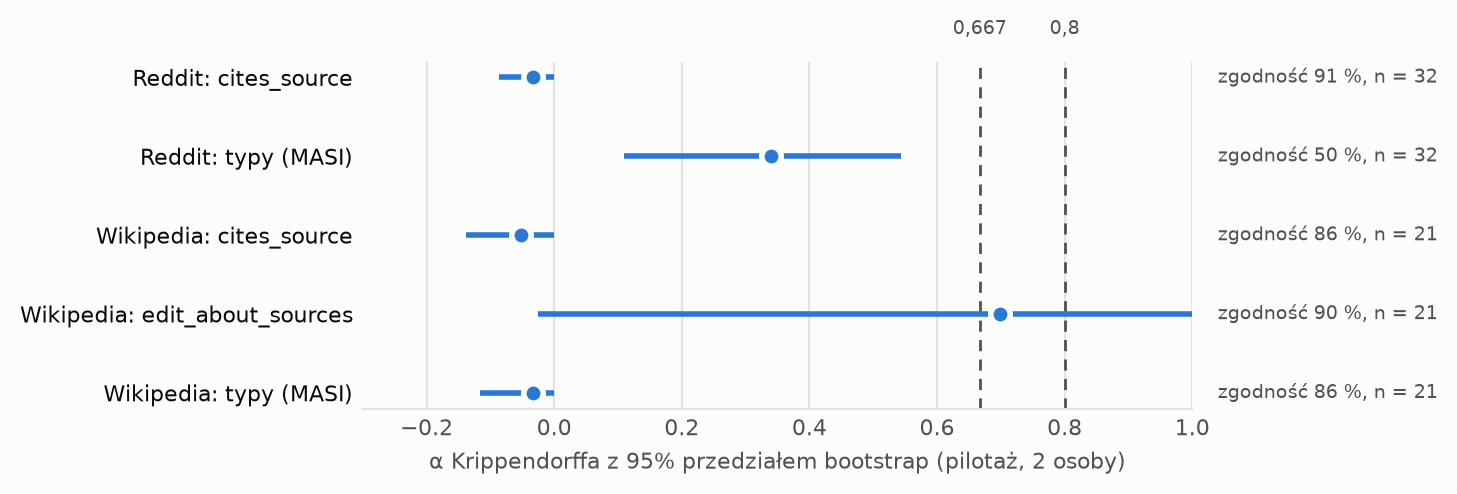
\includegraphics[width=0.85\linewidth]{preprint_agreement.png}
\caption{Zgodność dwóch osób w pilotażu: $\alpha$ Krippendorffa z 95\% przedziałem i progi 0,667 oraz 0,8.}
\label{fig:zgodnosc}
\end{figure}

\section{Walidacja instrumentów AI}
% 1,2 s., inżynier pipelinu. Tezy: trzy zamrożone instrumenty, jeden test (commit 33ff729);
% Reddit: GLiNER \resTestGlinerRedditCitesF, czułość \resTestGlinerRedditCitesRecall, typy \resTestGlinerRedditMasi,
% McNemar \resMcnemarRedditZeroshotGlinerP; v1 nie czyta linku (\resErrorsVoneUrlShare błędów);
% Wikipedia: wynik negatywny (\resTestGlinerWikipediaCitesF); zależność od annotatora
% (\resTestGlinerRedditMasiIS a \resTestGlinerRedditMasiJP); błąd różnicowy; wybór GLiNER do H1-B.
\dopisania{walidacja instrumentów (inżynier pipelinu)}

\begin{figure}[htbp]
\centering
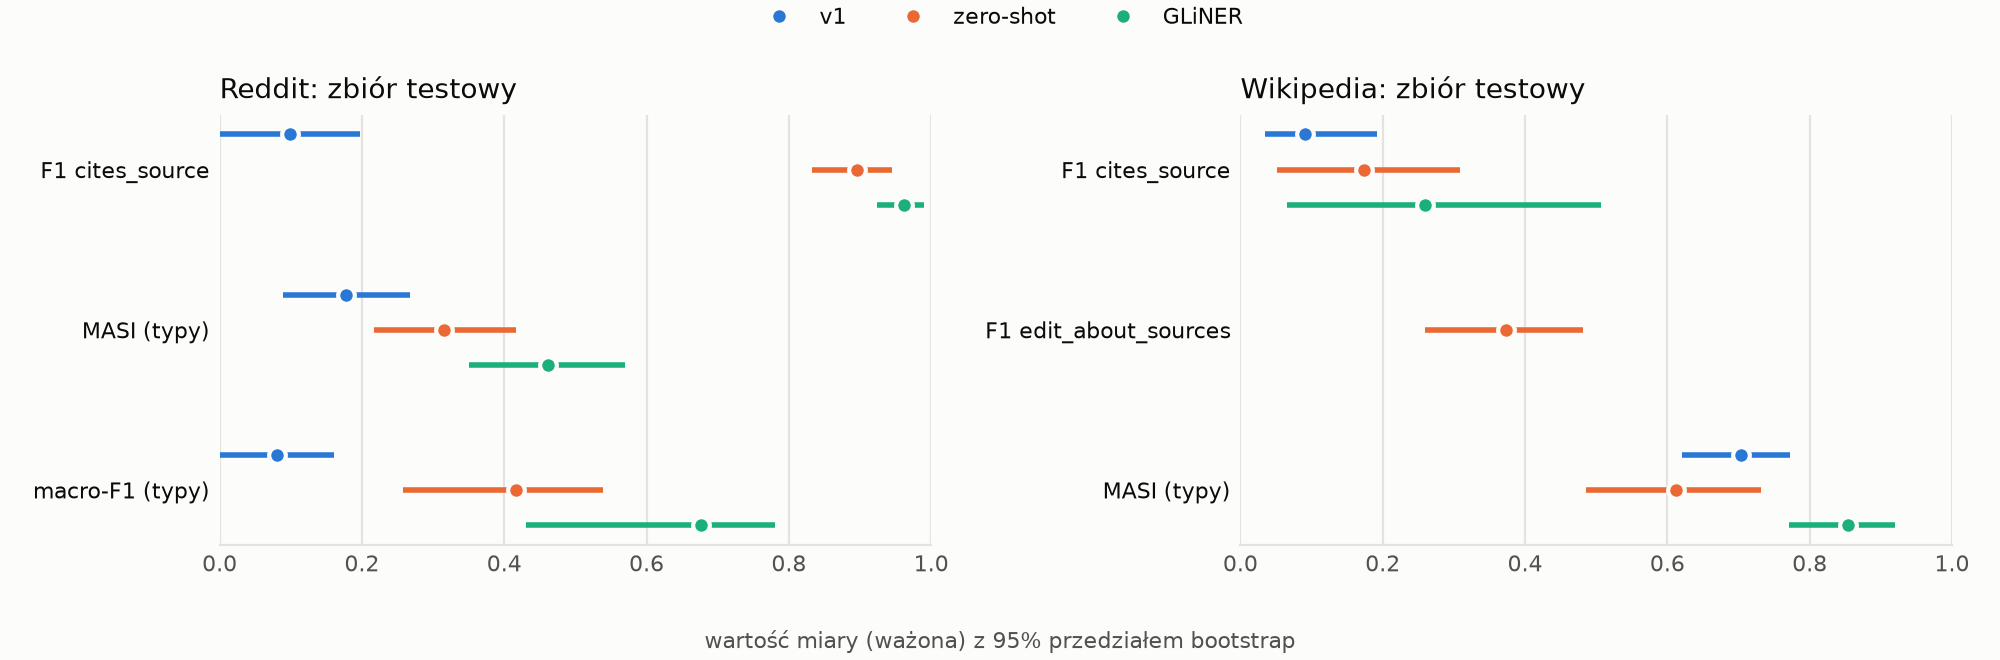
\includegraphics[width=\linewidth]{preprint_instruments.png}
\caption{Metryki trzech instrumentów na zbiorze testowym, ważone, z 95\% przedziałami bootstrap.}
\label{fig:instrumenty}
\end{figure}

\begin{table}[htbp]
\centering
\caption{Wyniki na zbiorze testowym (jeden przebieg na zamrożonych instrumentach).}
\label{tab:test}
\tabela{test_metrics}
\end{table}

\section{Wyniki}
\subsection{H1: zaufanie do konsensusu naukowego}
% 0,8 s., inżynier analityk. Tezy: H1-A się nie odbyło; H1-B na \resHoneBCiting postach:
% konsensus \resHoneBConsensusOr (p = \resHoneBConsensusP), alternatywne \resHoneBAlternativeOr
% (p = \resHoneBAlternativeP); surowe udziały w kierunku hipotezy, ale r/conspiracy rośnie
% z \resHoneConspiracyShareTwothousandeight do \resHoneConspiracyShareTwothousandeighteen; dekompozycja
% (eksploracyjna): alternatywne \resHoneBAlternativeShiftTotal, w tym skład \resHoneBAlternativeShiftComposition.
\dopisania{wyniki H1 (inżynier analityk)}

\begin{figure}[htbp]
\centering
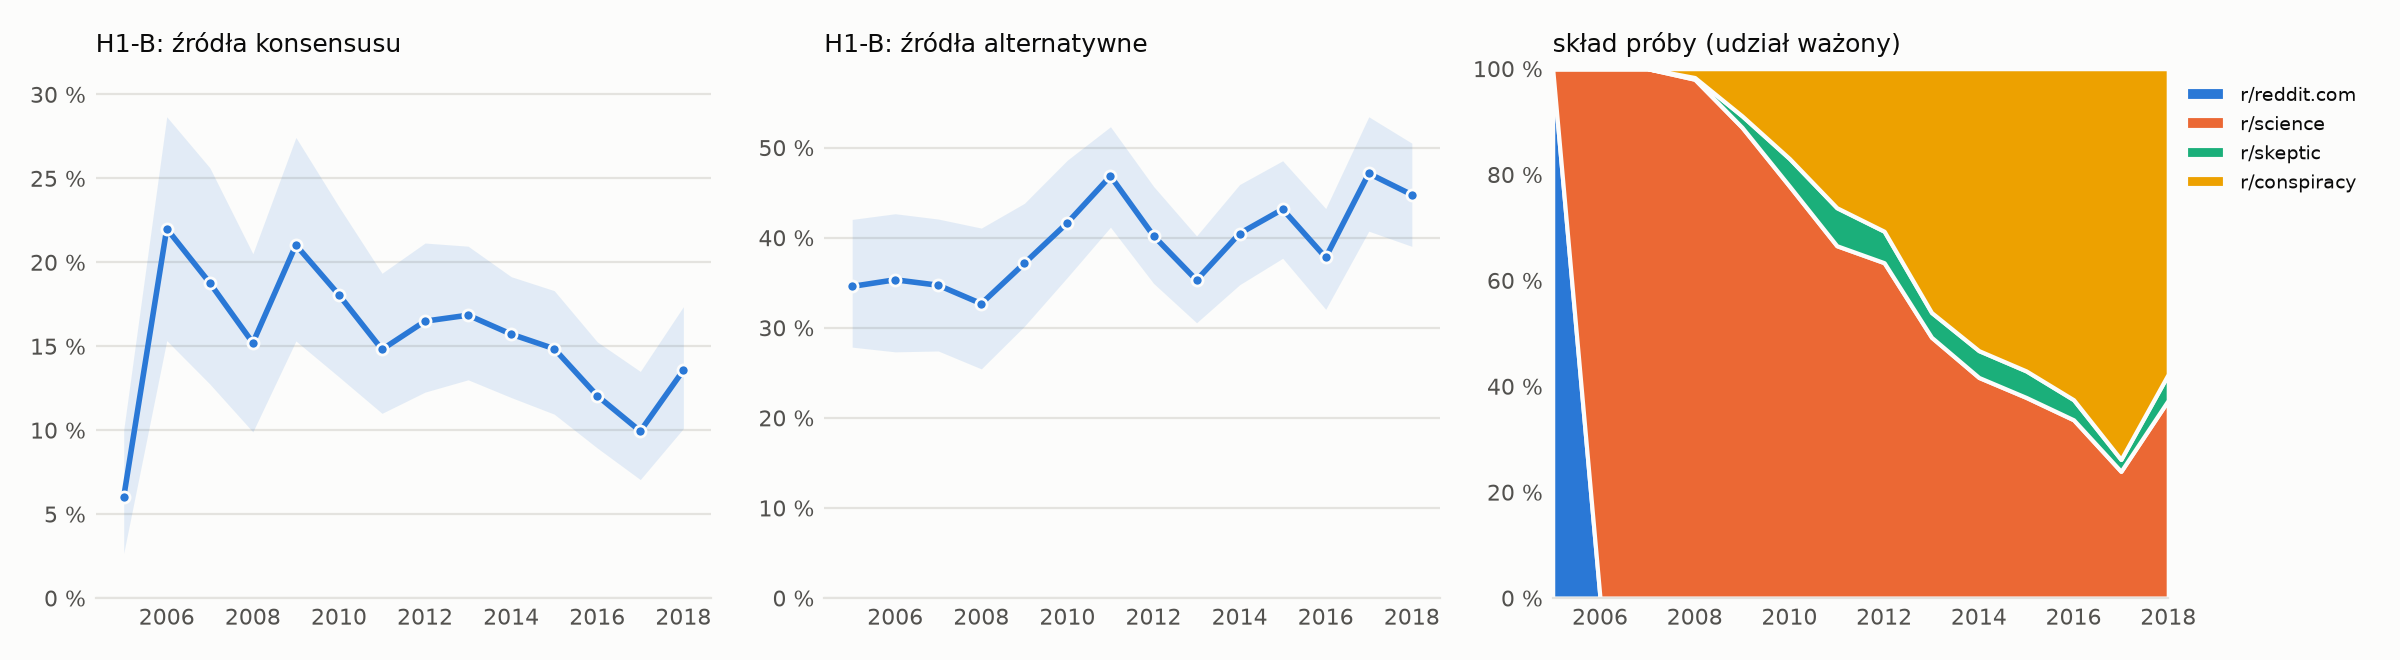
\includegraphics[width=\linewidth]{preprint_h1.png}
\caption{H1-B: roczne udziały źródeł konsensusu i alternatywnych wśród postów z powołaniem (z 95\% przedziałami) oraz skład próby według subredditu.}
\label{fig:h1}
\end{figure}

\begin{table}[htbp]
\centering
\caption{H1-B: iloraz szans na rok z efektami stałymi subredditu; $p$ jednostronne w kierunku hipotezy.}
\label{tab:h1b}
\szeroka{h1b}
\end{table}

\subsection{H2: źródła alternatywne w Wikipedii}
% 0,8 s., inżynier analityk. Tezy: test preregistrowany \resHtwoOr (p = \resHtwoP),
% \resHtwoAlternativeLinks{} z \resHtwoLinks{} linków; wrażliwości nieistotne (\resHtwoWithoutCovidP,
% permutacja \resHtwoPermutationP); \resHtwoOfficialLinks{} linków to konta WHO i GIS, link WHO
% dodany \resHtwoWhoRepeats{} razy; według właściciela 2 linki, test dokładny \resHtwoExactP.
\dopisania{wyniki H2 (inżynier analityk)}

\begin{figure}[htbp]
\centering
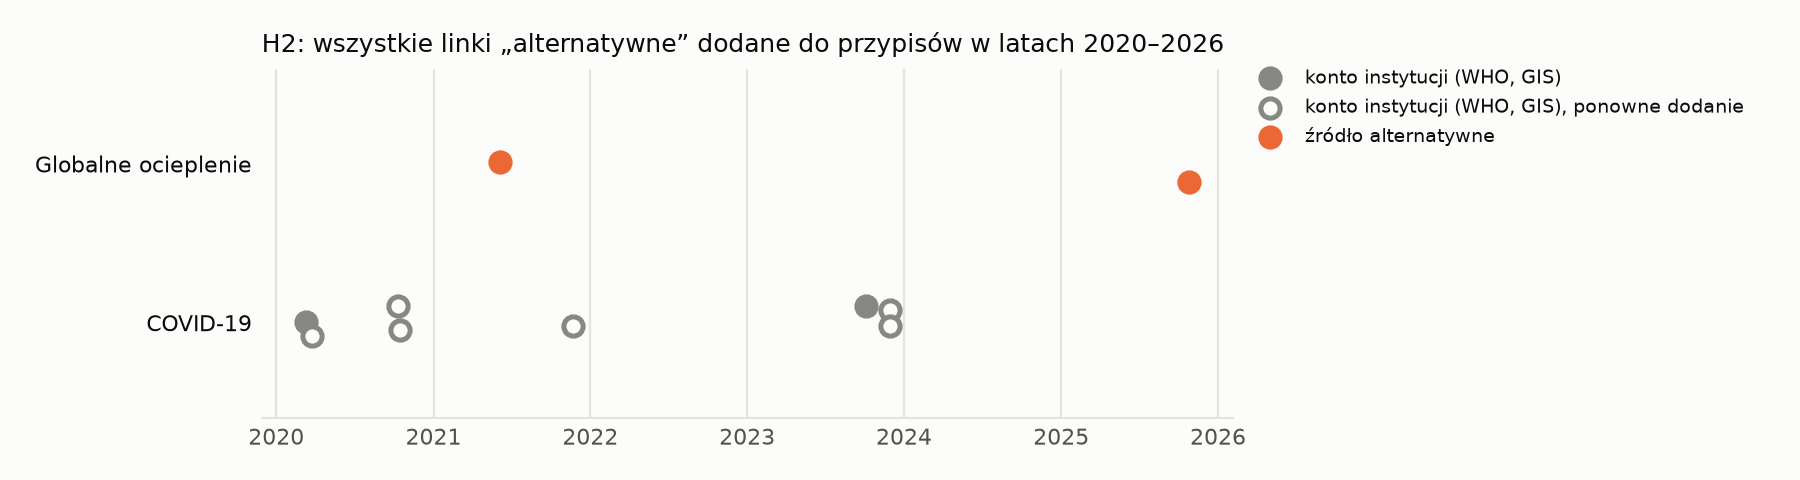
\includegraphics[width=\linewidth]{preprint_h2.png}
\caption{H2: wszystkie linki zaklasyfikowane jako alternatywne według domeny, według właściciela konta; puste punkty to ponowne dodania tego samego linku.}
\label{fig:h2}
\end{figure}

\begin{table}[htbp]
\centering
\caption{H2: test z preregistracji, analizy odporności i sprawdzenie pomiaru.}
\label{tab:h2}
\tabela{preprint_h2}
\end{table}

\section{Dyskusja i ograniczenia}
% 0,7 s., lead i analityk. Tezy: co dane rozstrzygają, a czego nie; lekcja o pomiarze
% (domena a właściciel konta, rewerty); ograniczenia (zgodność ludzi, etykiety wspomagane przez AI,
% błąd instrumentu, korelacja a przyczynowość, zmiany w obrębie subredditu, 8 stron);
% preregistracja v2 i analiza mocy jako dalsze prace.
\dopisania{dyskusja i ograniczenia (lead badawczy i inżynier analityk)}

\section{Odtwarzalność, dane i użycie AI}
% 0,3 s. Tezy: repozytorium, commit, polecenia make, preregistracje z commitami; data statement;
% użycie AI zgodne z faktami (kod i testy, etykiety wstępne JP zatwierdzone przez JP, lista domen,
% propozycje przyczyn błędów, pakiet wyników i szkic struktury; tekst napisali autorzy).
\dopisania{odtwarzalność, data statement i ujawnienie AI (inżynier danych i wszyscy)}

\begin{thebibliography}{99}
\bibitem{cohen1960} J.~Cohen. A coefficient of agreement for nominal scales. \textit{Educational and Psychological Measurement}, 20(1):37--46, 1960.
\bibitem{feinstein1990} A.~R. Feinstein, D.~V. Cicchetti. High agreement but low kappa: I.~The problems of two paradoxes. \textit{Journal of Clinical Epidemiology}, 43(6):543--549, 1990.
\bibitem{firth1993} D.~Firth. Bias reduction of maximum likelihood estimates. \textit{Biometrika}, 80(1):27--38, 1993.
\bibitem{kendall1938} M.~G. Kendall. A new measure of rank correlation. \textit{Biometrika}, 30(1/2):81--93, 1938.
\bibitem{krippendorff2004} K.~Krippendorff. \textit{Content Analysis: An Introduction to Its Methodology}. Wyd.~2. Sage, 2004.
\bibitem{laurer2024} M.~Laurer, W.~van Atteveldt, A.~Casas, K.~Welbers. Less annotating, more classifying: Addressing the data scarcity issue of supervised machine learning with deep transfer learning and BERT-NLI. \textit{Political Analysis}, 32(1):84--100, 2024.
\bibitem{mcnemar1947} Q.~McNemar. Note on the sampling error of the difference between correlated proportions or percentages. \textit{Psychometrika}, 12(2):153--157, 1947.
\bibitem{passonneau2006} R.~Passonneau. Measuring agreement on set-valued items (MASI) for semantic and pragmatic annotation. W: \textit{Proceedings of LREC 2006}, 2006.
\bibitem{zaratiana2024} U.~Zaratiana, N.~Tomeh, P.~Holat, T.~Charnois. GLiNER: Generalist model for named entity recognition using bidirectional transformer. W: \textit{Proceedings of NAACL 2024}, 2024.
\end{thebibliography}

\end{document}
